\newpage
\subsection{The katz-eig algorithm}\label{sec:background:theory:katzeig}

\Warning[TODO]{ Detailed introduction/description! }

The original algorithm \cite{katz1953new} is a link prediction algorithm. A short description of how the algorithm works will follow.

If $A$ is the interaction matrix then this the algorithm proposed:

\begin{equation}
    P = \sum_{t=1}^{\infty} \beta^t A^t
\end{equation}

Here $A^t$ can be seen as the $t$:th link value and $\beta$ signifies the diminishing return for links further away.

\Warning[TODO]{ Example run of the algorithm! }

As an additional modification the algorithm used in this thesis doesn't operate directly on $A$, but operates on a $k$ rank approximation of $A$.

% Originally introduced by \cite{katz1953new}, described and used by \cite{liben2007link}.

Concretely the \textit{katz-eig} algorithm follow these steps:

\begin{enumerate}
    \item Construct $U, S, V$ so $U * S * V'$ forms a rank $k$ approximation of $A$. Let $S_0 = S$.

    \item At each iteration $t = 1, \ldots, t_{max}$ perform:

        \begin{enumerate}
            \item $S_t = S_{t - 1} + \beta^t * S_{t - 1}^t$
        \end{enumerate}

        Repeat until convergence.

    \item Predicted user-item interaction is given by $P = U * S_{t_{max}} * V'$.

\end{enumerate}

There are two parameters to the algorithm: $\beta$ and $k$.


\subsubsection{Runtime exmple}

This is a runtime example for \textit{katz-eig} using a simple interaction matrix \eqref{eq:exA_katz}, which is the same matrix as in the example for \textit{link-analysis} (see \sectionref{sec:background:theory:linkanalysis}).

\begin{equation}\label{eq:exA_katz}
  A = \kbordermatrix{
    &    i_1 & i_2 & i_3 & i_4 \\
    u_1 & 0   & 1   & 0   & 1  \\
    u_2 & 0   & 1   & 1   & 1  \\
    u_3 & 1   & 0   & 1   & 0
  }
\end{equation}

This example uses $K = 2$, $\beta = 0.1$ and is run for $t_{max} = 3$ iterations.

Firstly a rank 2 SVD approximation is created
\[
U = \begin{pmatrix}
    -0.5592 &  0.4472 \\
    -0.7805 &  0.0000 \\
    -0.2796 & -0.8944 \\
\end{pmatrix},
\;
S = \begin{pmatrix}
    2.1889  &      0 \\
         0  & 1.4142
\end{pmatrix},
\;
V = \begin{pmatrix}
   -0.1277 & -0.6325 \\
   -0.6120 &  0.3162 \\
   -0.4843 & -0.6325 \\
   -0.6120 &  0.3162
\end{pmatrix}
\]

\[
    U * S * V' = \begin{pmatrix}
       -0.2436 &  0.9491  & 0.1928 &  0.9491 \\
        0.2182 &  1.0455  & 0.8273 &  1.0455 \\
        0.8782 & -0.0254  & 1.0964 & -0.0254
    \end{pmatrix}
    \approx
    A = \begin{pmatrix}
        0   & 1   & 0   & 1 \\
        0   & 1   & 1   & 1 \\
        1   & 0   & 1   & 0
    \end{pmatrix}
\]

Initially $S_0$ = $S$. Then $S_t$ is calculated iteratively
\[
    S_1 = \begin{pmatrix}
        0.2189 &    0 \\
        0      & 0.1414
    \end{pmatrix},
    \;
    S_2 = \begin{pmatrix}
        0.2668 &    0 \\
        0      & 0.1614
    \end{pmatrix},
    \;
    S_3 = \begin{pmatrix}
        0.2773 &    0 \\
        0      & 0.1642
    \end{pmatrix}
\]

until convergence or as in our case $t_{max} = 3$. The recommendations are then given by
\[
    U * S_3 * V' = \kbordermatrix{
        &    i_1 & i_2 & i_3 & i_4 \\
        u_1 &   -0.0266 &  0.1181 &  0.0286 &  0.1181 \\
        u_2 &    0.0276 &  0.1324 &  0.1048 &  0.1324 \\
        u_3 &    0.1028 &  0.0010 &  0.1305 &  0.0010
    }
\]

After removing the the items users already have interacted with in $A$, the prediction matrix $P$ becomes
\[
    P = \kbordermatrix{
        &    i_1 & i_2 & i_3 & i_4 \\
        u_1 &   -0.0266 &  0      &  \mathbf{0.0286} &  0      \\
        u_2 &    \mathbf{0.0276} &  0      &  0      &  0      \\
        u_3 &    0      &  \mathbf{0.0010} &  0      &  \mathbf{0.0010}
    }
\]

\Figureref{fig:ex_graph_link_rec} is a visualization of the most recommended items.

\begin{figure}[h!]
    \centering
    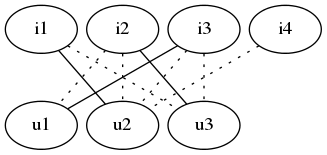
\includegraphics[width=0.3\linewidth]{fig/example_run/item_user_graph_katz_rec.png}
    \caption{A graph representing the most recommended item for each user. The dotted lines represent previous interactions.}
    \label{fig:ex_graph_katz_rec}
\end{figure}

\FloatBarrier

